\section{\textbf{IBM Model 2}}

\begin{algorithm*}[ht]
  \caption{The parameter estimation algorithm for IBM Model 2 for partially-observed data}
  \label{algo:ibm2}
  \KwIn{A training corpus $(s^{(k)}, e^{(k)})$ for $k=1\dots n$, where $s^{(k)}=s_1^{(k)}\dots s_{m_k}^{(k)}$, $e^{(k)}=e_1^{(k)}\dots e_{l_k}^{(k)}$. An integer $N=5$ specifying the number of iterations of training.}
  Initialization $t(s|e)$ as the last set of parameters (after $5$ iterations) produced by IBM Model 1\;
  Initialization $q(j|i,l,m)=\frac{1}{l+1}$\;
  \For{$step=1$ to $N$}
  {
    Set all counts $c(\dots)=0$\;
    \For{$k=1$ to $n$}
    {
        \For{$i=1$ to $m_k$}
        {
            \For{$j=0$ to $l_k$}
            {
                $c\left(e_{j}^{(k)}, s_{i}^{(k)}\right) \leftarrow c\left(e_{j}^{(k)}, s_{i}^{(k)}\right)+\delta(k, i, j), \ c\left(e_{j}^{(k)}\right)\leftarrow c\left(e_{j}^{(k)}\right)+\delta(k, i, j)$\;
                $c\left(j | i, l_{k}, m_{k}\right) \leftarrow c\left(j | i, l_{k}, m_{k}\right)+\delta(k, i, j), \ c\left(i, l_{k}, m_{k}\right) \leftarrow c\left(i, l_{k}, m_{k}\right)+\delta(k, i, j)$\;
                where $\delta(k, i, j)=\frac{q\left(j | i, l_{k}, m_{k}\right) t\left(s_{i}^{(k)} | e_{j}^{(k)}\right)}{\sum_{j=0}^{l_{k}} q\left(j | i, l_{k}, m_{k}\right) t\left(s_{i}^{(k)} | e_{j}^{(k)}\right)}$
            }
        }
    }
    Set $t(s | e)=\frac{c(e, s)}{c(e)}$, $q(j|i,l,m)=\frac{c(j|i,l,m)}{c(i,l,m)}$\;
  }
  \KwOut{parameters $t(s|e)$.}
\end{algorithm*}


\subsection{\textbf{Description of IBM Model 2}}

\subsubsection{\textbf{Comparison with IBM Model 1}}

The IBM Model 2 is very similar to IBM Model 1 except for it extends the implementation of the EM algorithm and has a set of new parameters. The main additional step is adapting the delta function to include $q(j|i,l,m)$ which represents the probability that $j$-th Spanish word is connected to the $i$-th English word given sentence length of $e$ and $s$ are $1$ and $m$ respectively.

IBM Model 2 outperforms IBM Model 1 because of the alignment parameter $q$. It can model the translation of a source sentence word in position $i$ to a target language sentence word in position $j$ using the alignment probability distribution.

\subsubsection{\textbf{Limitations of IBM Model 2}}

IBM Model 2 still uses only word-to-word translations between languages where as in reality many translations could only be achieved if group of words (phrase) are translated together. Also it sometimes maps an English (target language) word too many times to other Spanish words (source language). 

\subsection{\textbf{Method Overview}}

\subsubsection{\textbf{High-Level Description of Implementation}}

My implementation of IBM Model 2 includes two parts: training and testing. The training part is done by running $5$ iterations of EM Algorithm. More details can be found in Algorithm~\ref{algo:ibm2}. The testing part includes reading parameters as well as testing corpora and assigning alignment to each sentences pair with the highest $q*t$ score, i.e. $a_{i}=\underset{j \in 0 \ldots l}{\arg \max } q(j | i, l, m) t\left(s_{i} | e_{j}\right)$.

\subsection{\textbf{Results}}

The result of my implementation matches the expected F1-Score. Details can be found in Table \ref{tab:ibm2}.

\begin{table}[ht]  %table 里面也可以嵌套tabular,只有tabular是不能加标题的
\centering  %表格居中
\caption{Performances of IBM Model 2}
\begin{tabular}{lcccc }
\hline
&    \textbf{Precision} & \textbf{Recall} & \textbf{F1-Score}  \\
\hline
 \textbf{Total} & 0.442 & 0.456 & 0.449 \\
\hline
\end{tabular}
\label{tab:ibm2}
\end{table}

% F1 Score

\subsection{\textbf{Discussions}}

\subsubsection{\textbf{Performances throughout iterations}}

% F1 Score changes vs iteration
% Compare with IBM Model 1

\begin{table}[ht]  %table 里面也可以嵌套tabular,只有tabular是不能加标题的
\centering  %表格居中
\caption{Performances of IBM Model 2}
\begin{tabular}{cccccc}
\hline
\textbf{IBM Model 1} &    \textbf{Precision} & \textbf{Recall} & \textbf{F1-Score} & \textbf{Growth Rate}  \\
\hline
  & 0.413 & 0.427 & 0.420 & - \\
 \hline
\textbf{Iterations} &    \textbf{Precision} & \textbf{Recall} & \textbf{F1-Score} & \textbf{Growth Rate}  \\
\hline
 \textbf{1} & 0.430 & 0.444 & 0.437 & \textbf{4.0\%} \\
 \hline
 \textbf{2} & 0.436 & 0.450 & 0.443 & 1.4\%\\
 \hline
 \textbf{3} & 0.439 & 0.454 & 0.446 & 0.68\%\\
 \hline
 \textbf{4} & 0.438 & 0.453 & 0.445 & -0.22\%\\
\hline
 \textbf{5} & 0.442 & 0.456 & 0.449 & 0.90\%\\
 \hline
 \textbf{6} & \textbf{0.443} & \textbf{0.457} & \textbf{0.450} & 0.22\%\\
 \hline
 \textbf{7} & 0.443 & 0.457 & 0.450 & 0.0\%\\
 \hline
 \textbf{8} & 0.442 & 0.456 & 0.449 & -0.22\%\\
 \hline
 \textbf{9} & 0.442 & 0.456 & 0.449 & 0.0\%\\
 \hline
 \textbf{10} & 0.442 & 0.457 & 0.449 & 0.0\%\\
\hline
\end{tabular}
\label{tab:ibm2iter}
\end{table}

The performances through the training process are given by the Table~\ref{tab:ibm2iter}. We can see from the table the following facts:
\begin{itemize}
    \item The performances of IBM Model 2 is a clear improvement compared with IBM Model 1. The first iteration gives a 4\% improvement over the final F1-Score of IBM Model 1. This is reasonable since our IBM Model 2's parameter $t(s|e)$ is initialized using the last set of parameters (after 5 iterations) produced by IBM Model 1 and IBM Model 2 introduced the alignment parameters $q$.
    \item Again, there is an interesting phenomenon that the growth rate is mostly always decreasing as the iteration goes. From iteration 2 to 5, the magnitude of improvement gradually decreases and even has a negative growth in iteration 4. But iteration 5 witnesses another improvement. 
    \item There is a bottleneck in the performance of IBM Model 2. After $6$ iterations, the performances almost arrives at its peak and will no longer increase. 
\end{itemize}

\subsubsection{\textbf{Examples of alignments}}

There are two misaligned word pairs in the figure~\ref{fig:align1}. "que" is misaligned to "hope" and "puedan" is misaligned to "use". Other than these two pairs, other word pairs are correctly aligned with each other. The accuracy is high enough to put it under the correctly aligned sentence category. The reason why this pair of sentences are aligned most correctly is that the sentences are in relatively simple grammatical structures. The alignments of these word pairs are one-to-one and the mapping of words is straight forward. Also, there are no complex phrases in the sentences. 

IBM Model 2 lacks the ability to translate phrases. It only uses lexical parameters and distortion parameters to calculate the alignments. Therefore, when sentence pairs do not have complicated phrases or sentence structure, the performance of the model tends to be high.

\begin{figure}[!ht]
    \centering
    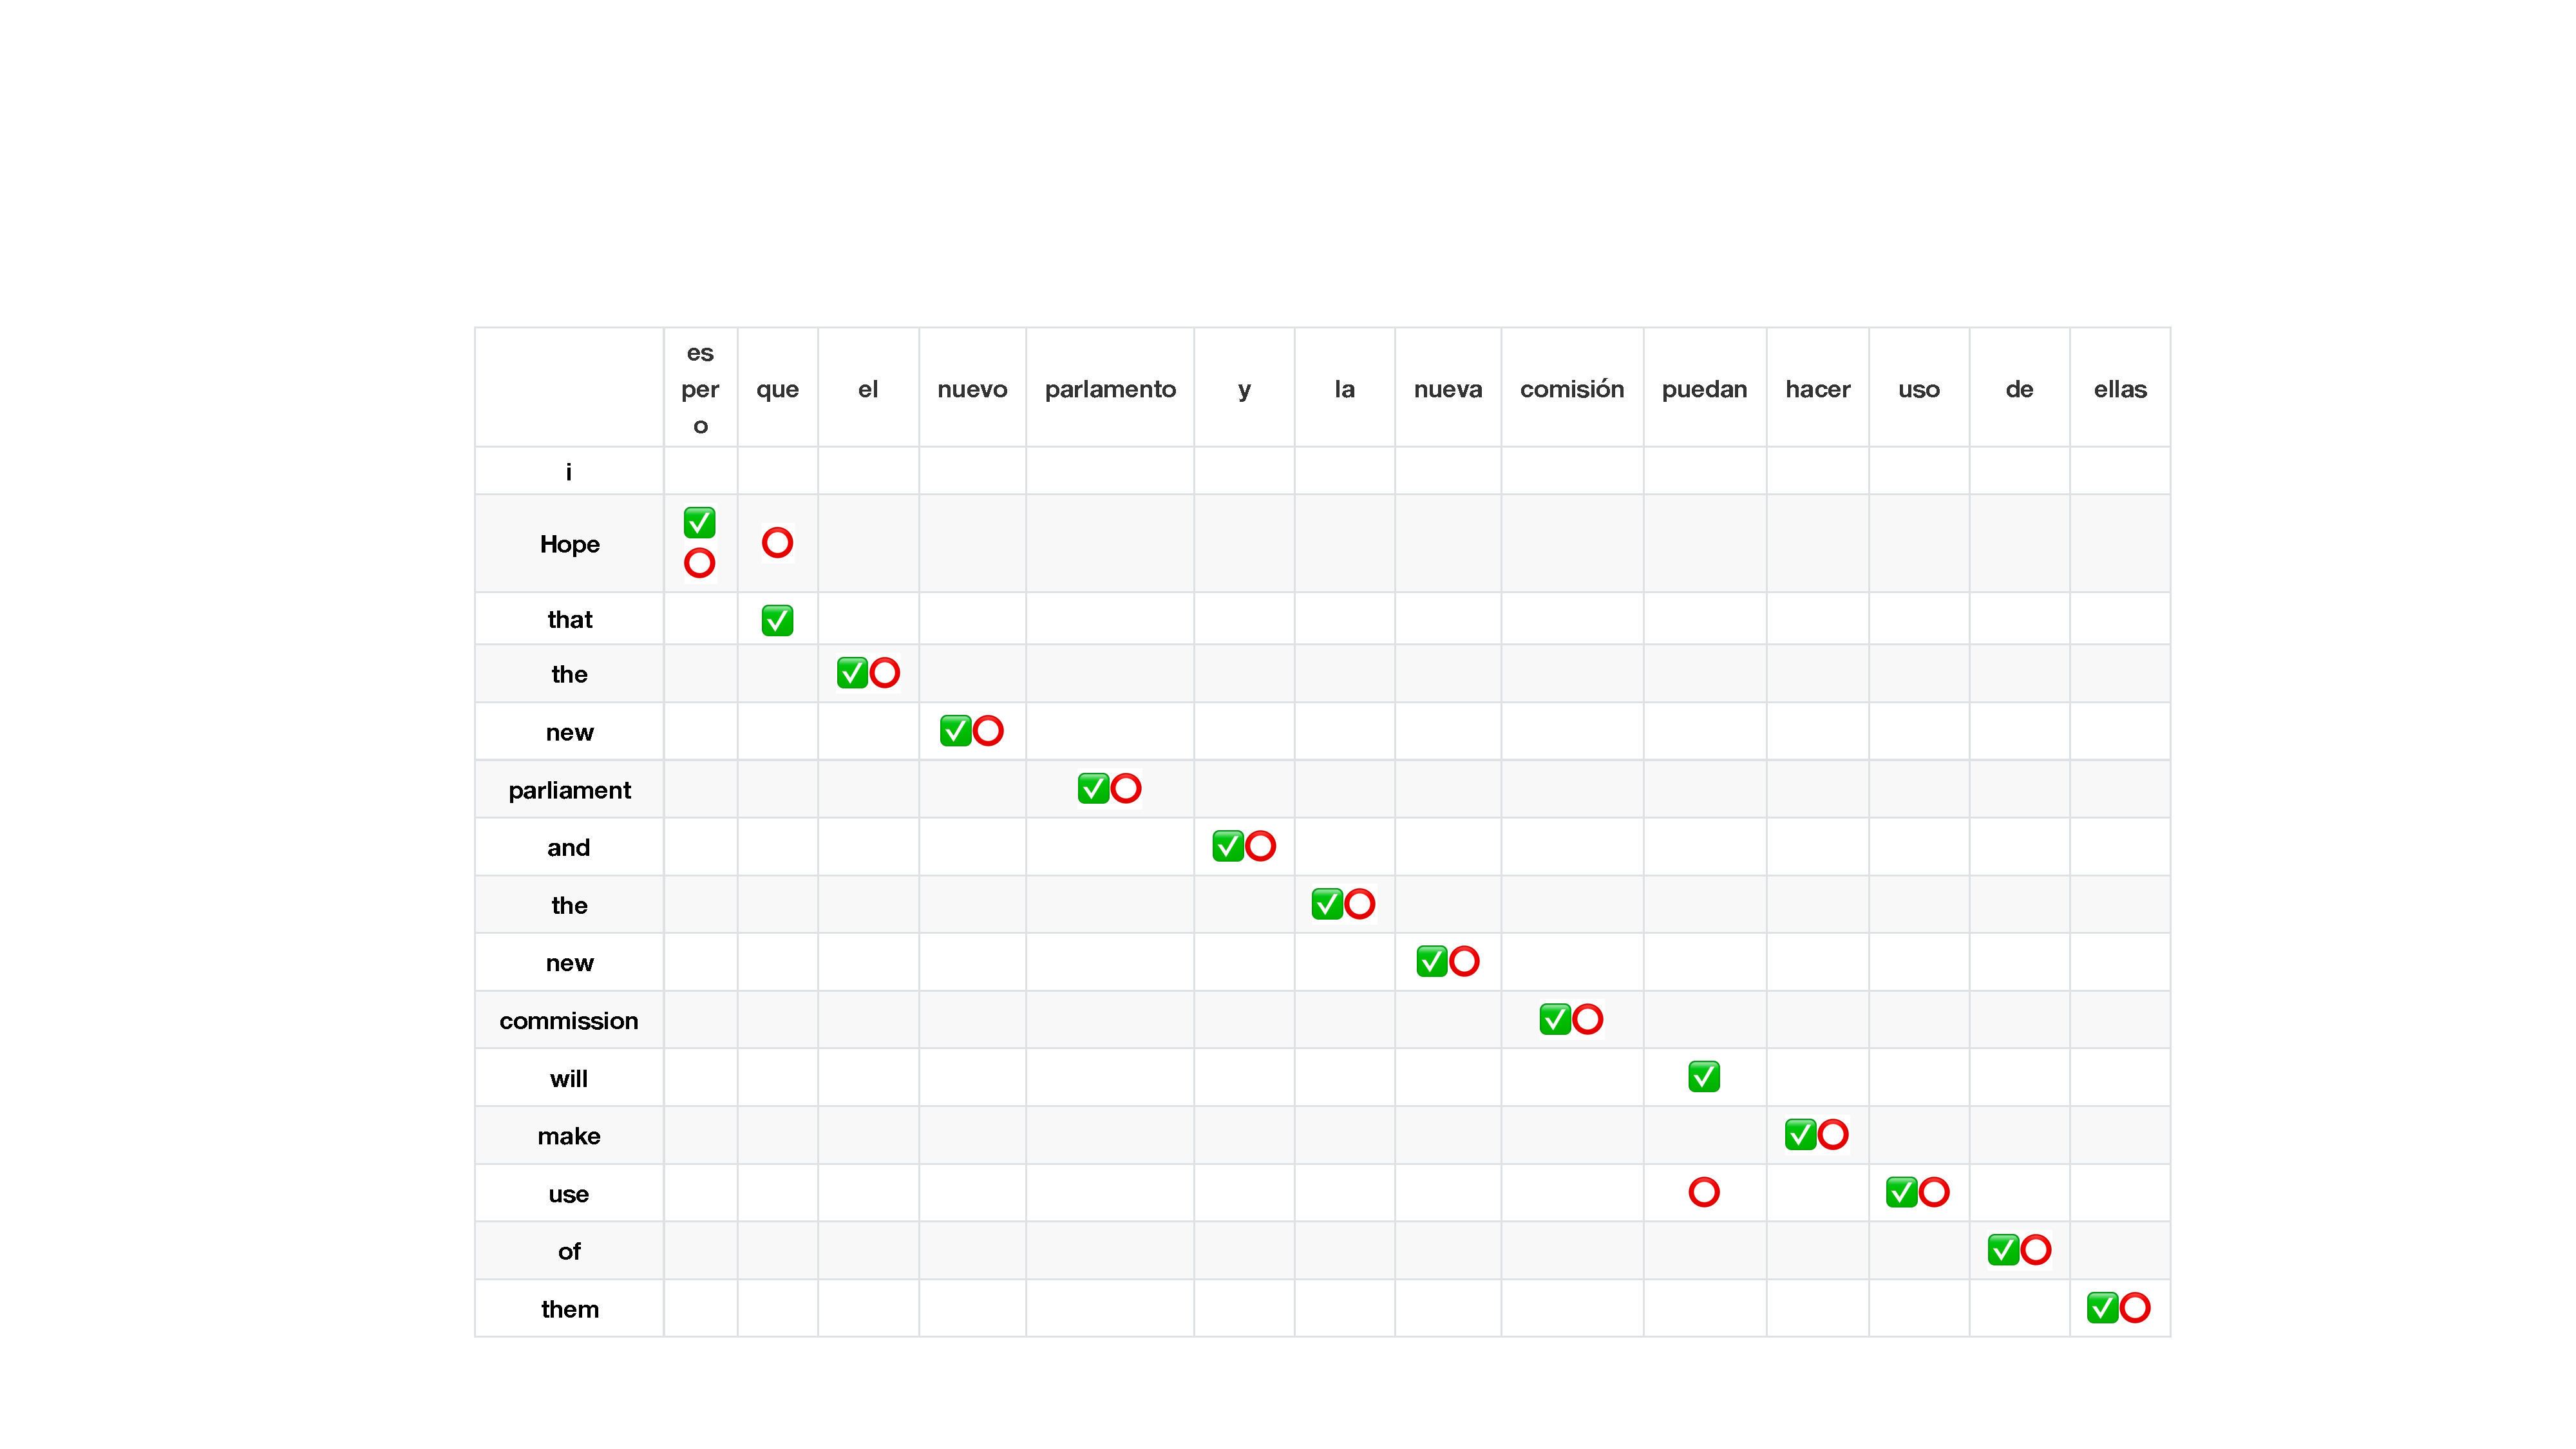
\includegraphics[width=0.47\textwidth]{files/figs/1.pdf}
    \caption[]%
    {\small An example of correctly aligned sentence. The red circle sign represents alignments generated by IBM Model 2 while the green tick sign represents the golden alignments for the sentence pair.}
    \label{fig:align1}
\end{figure}

In figure~\ref{fig:align2}, a misaligned example is shown. Different from the correctly aligned sentence, this sentence has a phrase "no reason not to" and its counterpart in Spanish "no razón para no". The Model clearly failed to catch the meaning of this phrase. This reveals the weakness of the model, which is not able to process phrases correctly.

\begin{figure}[!ht]
    \centering
    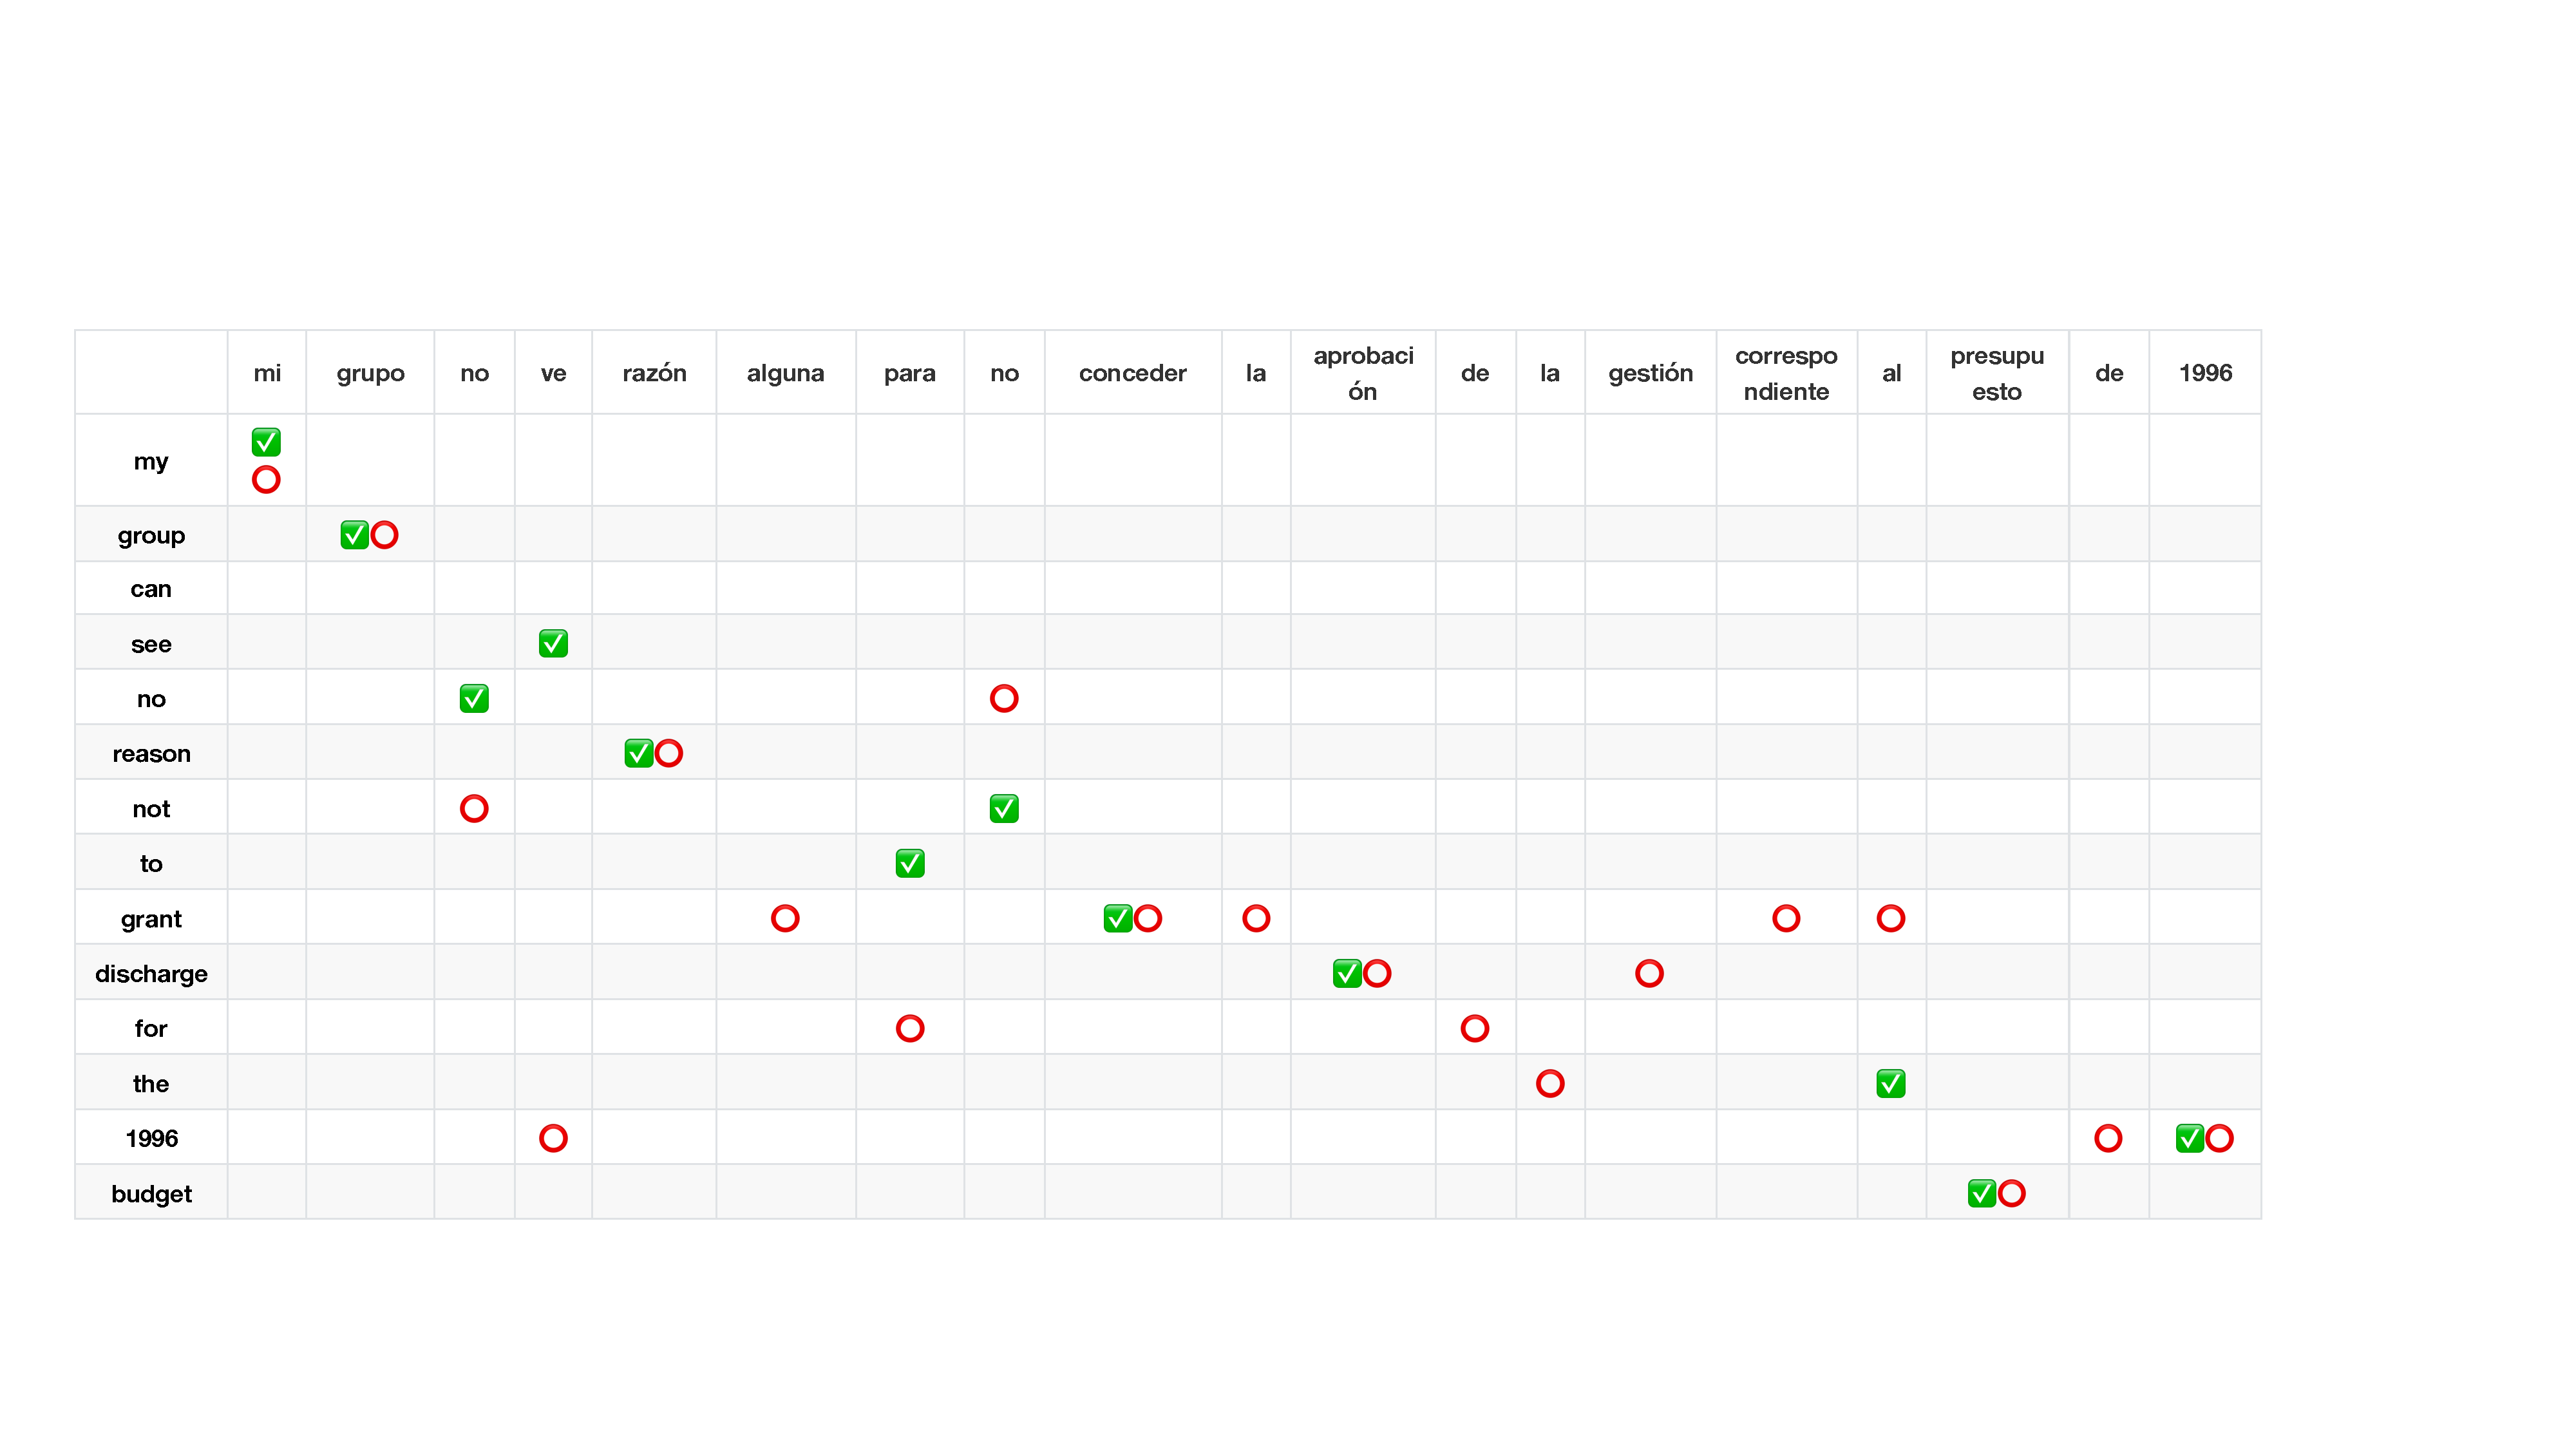
\includegraphics[width=0.5\textwidth]{files/figs/2.pdf}
    \caption[]%
    {\small An example of misaligned sentence. }
    \label{fig:align2}
\end{figure}

% Use the type of table/graph as in the slides or in the instructions, show two correctly aligned examples + two misaligned examples. Discuss the examples.
